\section{Results}

\subsection{Study Cohort}

The study cohort comprised 48,354 hospital admissions among 29,577 unique
adult patients who met the predefined clinical cohort criteria across six
Israeli general hospitals during the study period from August 2022 through
December 2025 (Table~\ref{tab:cohort}). Admissions were distributed across
all six participating hospitals, with center-specific sample sizes ranging
from 4,478 to 11,024 admissions.

The study population had a mean age of 71.9 years (median, 73.3), and
54.3\% were male. The median length of stay was 5.55 days. Among relevant
admissions, 35.3\% had a documented diabetes diagnosis, 74.7\% met the
recurrent-hyperglycemia criterion, and 60.2\% had at least one extreme
glucose measurement. Among admissions with a documented diabetes diagnosis,
50.3\% also met the recurrent- or extreme-hyperglycemia criterion.
Conversely, only 21.5\% of admissions meeting a hyperglycemia criterion
had a documented diabetes diagnosis, indicating that a substantial
proportion of the cohort represented clinically significant inpatient
hyperglycemia without a recorded diabetes diagnosis.

The pre-intervention period contributed 21,605 admissions among 17,002
patients, and the post-intervention period 16,182 admissions among 11,201
patients.

% Table 1: Cohort characteristics
\begin{table}[t]
\centering
\caption{Characteristics of the multicenter study cohort.}
\label{tab:cohort}

\begin{tabularx}{\textwidth}{
>{\raggedright\arraybackslash}X
>{\raggedleft\arraybackslash}p{0.34\textwidth}
}
\toprule
Characteristic & Value \\
\midrule

Hospitals & 6 \\
Admissions & 48,354 \\
Unique patients & 29,577 \\
Age, mean (median), years & 71.9 (73.3) \\
Male sex & 54.3\% \\
Length of stay, median, days & 5.55 \\
30-day mortality & 9.58\% \\

\midrule

Documented diabetes diagnosis & 35.3\% \\
Recurrent hyperglycemia & 74.7\% \\
Extreme glucose ($\geq250$ mg/dL) & 60.2\% \\
Hyperglycemia among admissions with diabetes & 50.3\% \\
Diabetes diagnosis among admissions with hyperglycemia & 21.5\% \\

\midrule

Pre-intervention cohort &
\makecell[r]{21,605 admissions\\17,002 patients} \\

Post-intervention cohort &
\makecell[r]{16,182 admissions\\11,201 patients} \\

\bottomrule
\end{tabularx}
\end{table}


\subsection{Guideline Adherence and Changes Following National Implementation}
\label{sec:adherence-results}

\subsubsection{Overall Guideline Adherence}

Adherence varied sharply across recommendations
(Table~\ref{tab:overall-adherence}), and the split followed the kind of
action required rather than its clinical weight. Single discrete actions on
admission were near-universal: SGLT2 discontinuation was complete ($1.00$)
and creatinine measurement almost so ($0.98$). Recommendations calling for
repeated insulin decisions across the stay were not: insulin following hyperglycemia
scored $0.15$, the two routine basal dosing components $0.21$ and $0.23$,
and bolus reduction after hypoglycemia $0.28$---all with a median of zero,
meaning the expected action was absent altogether in most eligible
admissions. Monitoring and admission medication management fell between
these extremes ($0.54$--$0.88$).

Adherence was largely independent of whether diabetes had been formally
documented. Among admissions with hyperglycemia in the first 48 hours, mean
adherence was $0.669$ where a diagnosis was recorded and $0.661$ where it
was not; the difference of $0.008$ reached significance only by virtue of
the sample size.

\begin{table}[t]
\centering
\caption{Overall adherence to assessed inpatient diabetes guideline recommendations
during the study period. Scores range from 0 (non-adherence) to 1 (complete
adherence).}
\label{tab:overall-adherence}

\begin{tabularx}{\textwidth}{
>{\raggedright\arraybackslash}X
l
r
r
}
\toprule
Guideline recommendation & Constraint & Mean & Median \\
\midrule

Admission glucose monitoring
    & Cyclic & 0.85 & 1.00 \\

Routine glucose monitoring
    & Cyclic & 0.88 & 0.98 \\

Glucose monitoring during corticosteroid therapy
    & Cyclic & 0.54 & 0.50 \\

BMI measurement on admission
    & Time & 0.87 & 1.00 \\

Creatinine measurement on admission
    & Time & 0.98 & 1.00 \\

Antidiabetic discontinuation on admission
    & Time & 0.66 & 0.86 \\

SGLT2 discontinuation on admission
    & Time & 1.00 & 1.00 \\

Basal insulin continuation on admission
    & Time & 0.66 & 1.00 \\

Insulin administration after hyperglycemia
    & Time & 0.15 & 0.00 \\

Antidiabetic discontinuation after hypoglycemia
    & Time & 0.89 & 1.00 \\

Basal dose reduction after hypoglycemia
    & Value & 0.87 & 1.00 \\

Bolus dose reduction after hypoglycemia
    & Value & 0.28 & 0.00 \\

Routine basal dosage (frequency)
    & Cyclic & 0.23 & 0.00 \\

Routine basal dosage (dose)
    & Value & 0.21 & 0.00 \\

\bottomrule
\end{tabularx}
\end{table}


\subsubsection{Changes in Adherence Following the Intervention}

Overall adherence rose from $0.682$ before the guideline to $0.703$ after
($p<0.001$; Figure~\ref{fig:adherence-trend}), with monthly scores trending
upward across the period. The absolute change is small, and its significance
reflects the number of admissions rather than the size of the shift.

Component-level changes were uneven (Table~\ref{tab:adherence-change}).
Glucose monitoring improved most: on admission from $0.78$ to $0.93$
($+0.15$), throughout the stay from $0.83$ to $0.94$ ($+0.11$), and during
corticosteroid treatment from $0.51$ to $0.58$ ($+0.07$). Discontinuation of
high-hypoglycemia-risk antidiabetic agents on admission rose from $0.62$ to
$0.75$ ($+0.13$). Gains in the insulin-management components were significant
but marginal ($+0.01$ to $+0.03$), leaving them close to their already low
baselines. Continuation of basal insulin on admission rose slightly but did
not survive correction ($p_{\mathrm{FDR}}=0.054$), nothing changed in dose
reduction after hypoglycemia, and SGLT2 discontinuation was already complete
in both periods.

Center-level trajectories ranged from improvement through no measurable
change to modest decreases, so the pooled increase conceals substantial
inter-hospital heterogeneity.

\begin{table}[t]
\centering
\caption{Changes in adherence to inpatient diabetes guideline recommendations
before and after the national implementation. Confidence intervals are
unadjusted 95\% confidence intervals for the absolute difference in mean
adherence ($\Delta$). Reported $p$-values were adjusted across component-level
comparisons using the Benjamini--Hochberg false discovery rate (FDR)
procedure.}
\label{tab:adherence-change}

\small

\begin{tabularx}{\textwidth}{
>{\raggedright\arraybackslash}X
rrrrr
}
\toprule
Guideline recommendation & Before & After & $\Delta$ & 95\% CI & $p_{\mathrm{FDR}}$ \\
\midrule

Admission glucose monitoring
    & 0.78 & 0.93 & +0.15 & [0.145, 0.154] & $<0.001$ \\

Routine glucose monitoring
    & 0.83 & 0.94 & +0.11 & [0.105, 0.113] & $<0.001$ \\

Glucose monitoring during corticosteroid therapy
    & 0.51 & 0.58 & +0.07 & [0.062, 0.087] & $<0.001$ \\

BMI measurement on admission
    & 0.86 & 0.89 & +0.03 & [0.015, 0.029] & $<0.001$ \\

Creatinine measurement on admission
    & 0.98 & 0.99 & +0.01 & [0.008, 0.014] & $<0.001$ \\

SGLT2 discontinuation on admission
    & 1.00 & 1.00 & 0.00 & -- & -- \\

Antidiabetic discontinuation on admission
    & 0.62 & 0.75 & +0.13 & [0.075, 0.192] & $<0.001$ \\

Basal insulin continuation on admission
    & 0.63 & 0.67 & +0.04 & [0.002, 0.089] & 0.054 \\

Insulin administration after hyperglycemia
    & 0.14 & 0.15 & +0.01 & [0.009, 0.020] & $<0.001$ \\

Antidiabetic discontinuation after hypoglycemia
    & 0.91 & 0.89 & -0.02 & [-0.197, 0.158] & 0.818 \\

Basal dose reduction after hypoglycemia
    & 0.87 & 0.88 & +0.01 & [-0.015, 0.034] & 0.497 \\

Bolus dose reduction after hypoglycemia
    & 0.33 & 0.26 & -0.07 & [-0.158, 0.029] & 0.210 \\

Routine basal dosage (frequency)
    & 0.21 & 0.24 & +0.03 & [0.027, 0.043] & $<0.001$ \\

Routine basal dosage (dose)
    & 0.19 & 0.22 & +0.03 & [0.021, 0.036] & $<0.001$ \\

\bottomrule
\end{tabularx}
\end{table}

\begin{figure}[t]
    \centering
    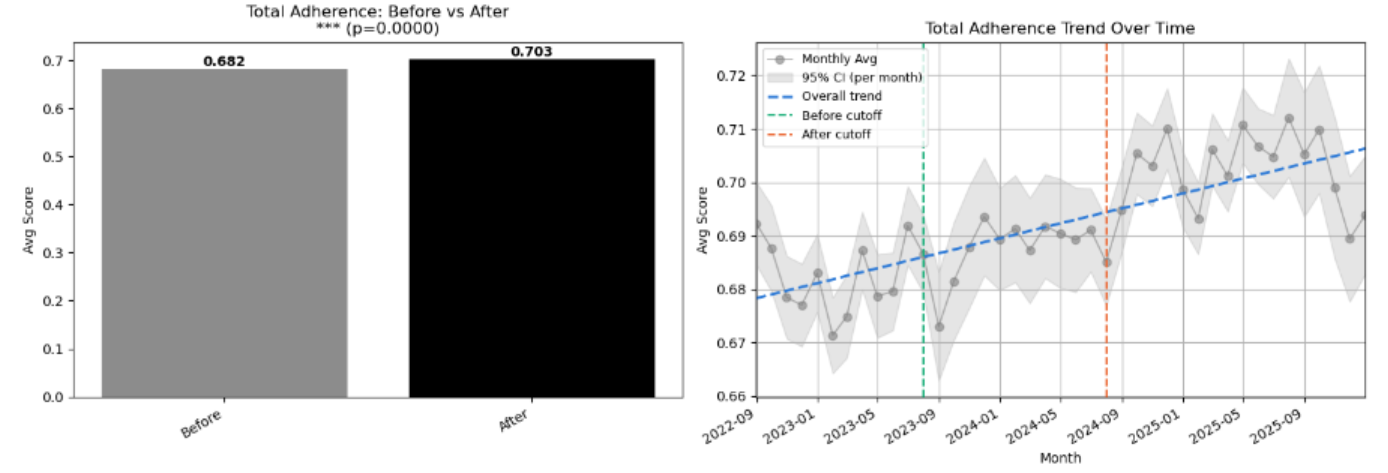
\includegraphics[width=\textwidth]{figures/adherence_trend.png}
    \caption{
    Changes in overall guideline adherence across the study period.
    \textbf{Left:} Mean overall adherence scores during the predefined
    pre-intervention (August 2022--July 2023) and post-intervention
    (August 2024--December 2025) periods.
    \textbf{Right:} Monthly mean overall adherence scores with 95\%
    confidence intervals across the study period. Vertical dotted lines
    delimit the transition/intervention period excluded from the primary
    pre--post comparison, and the dashed line indicates the overall
    temporal trend.
    }
    \label{fig:adherence-trend}
\end{figure}


\subsection{Guideline Adherence and Clinical Outcomes}

\subsubsection{Overall Adherence and 30-Day Mortality}

Higher adherence was associated with lower 30-day mortality
(Figure~\ref{fig:adherence-mortality}). Survivors had a higher mean
adherence score than those who died ($0.693$ vs.\ $0.652$, $p<0.001$), and
mortality fell across adherence strata, from 11\% at the bottom to roughly
3\% among admissions scoring $0.90$--$1.00$. On the continuous score, each
$0.1$-point increase carried $16.8\%$ lower odds of death (OR $=0.832$,
95\% CI $[0.811, 0.853]$), so the association is graded rather than
threshold-like. Adjusting for age, sex, comorbidity burden and hospital left
it intact (adjusted OR $=0.757$, 95\% CI $[0.727, 0.788]$, per
one-standard-deviation increase).

\begin{figure}[t]
    \centering
    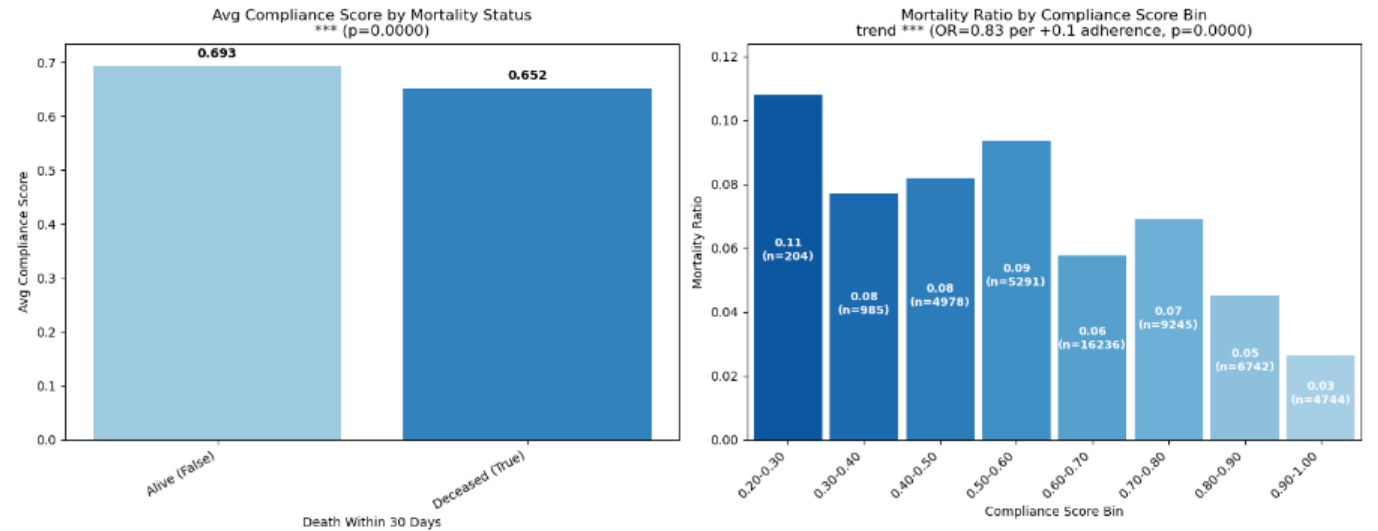
\includegraphics[width=\textwidth]{figures/adherence_mortality.png}
    \caption{
    Association between overall guideline adherence and 30-day mortality.
    \textbf{Left:} Mean overall adherence scores among patients who survived
    and those who died within 30 days.
    \textbf{Right:} Observed 30-day mortality rates across strata of overall
    adherence score; the number of admissions in each stratum is shown
    within the corresponding bar. Strata containing fewer than 30 admissions
    are not shown. The trend statistic reported above the panel is from
    logistic regression on the continuous adherence score, not on the
    binned values, and is expressed as the odds ratio per $0.1$-point
    increase in adherence.
    }
    \label{fig:adherence-mortality}
\end{figure}

\subsubsection{Insulin-Guideline Adherence and Hypoglycemia}

Adherence to the insulin-management recommendations showed negligible
correlation with subsequent hypoglycemic burden---measured as the proportion
of hospitalization days with events---for both hypoglycemia ($r=0.052$) and
severe hypoglycemia ($r=0.056$; $n=40{,}719$).

\subsection{Identifying Outcome-Associated Guideline Recommendations}

One model was fitted per complication per observation window, with adherence
and baseline covariates entered jointly (Table~\ref{tab:firth-summary}).
Between 9 and 34 predictors were retained per outcome, but the number
surviving all three window definitions ranged from none to 32, tracking
event frequency: mortality yielded the most robust predictors and the rarer
complications few or none. Mortality therefore serves as the worked example
below.

\begin{table}[t]
\centering
\caption{Summary of the bias-reduced (Firth) regression models.
Positive-event counts are shown for each observation-window definition.
Retained features denote predictors that remained significant after FDR
correction and pruning of highly correlated features. Robust features
remained statistically significant with the same effect direction across
all three observation-window definitions. MI, myocardial infarction;
AKI, acute kidney injury.}
\label{tab:firth-summary}

\begin{tabularx}{\textwidth}{
>{\raggedright\arraybackslash}X
ccccc
}
\toprule
Outcome & 24 h & 48 h & 72 h &
Retained & Robust \\
\midrule

Inpatient MI & 175 & 125 & 90 & 13 & 0 \\
30-day mortality & 3130 & 3130 & 2793 & 34 & 32 \\
Hyperglycemia & 8565 & 2153 & 1135 & 13 & 0 \\
Hyperosmolarity & 75 & 58 & 45 & 9 & 0 \\
Hypoglycemia & 2437 & 1742 & 1234 & 24 & 0 \\
Infection & 898 & 475 & 291 & 12 & 2 \\
Ketoacidosis & 46 & 33 & 25 & 9 & 0 \\
Inpatient AKI & 1362 & 901 & 655 & 21 & 5 \\
Severe hyperglycemia & 10019 & 4328 & 2376 & 28 & 8 \\
Severe hypoglycemia & 1686 & 1207 & 851 & 22 & 0 \\

\bottomrule
\end{tabularx}
\end{table}

\subsubsection{Component-Level Feature Importance}

Figure~\ref{fig:death-importance} shows the mortality profile. The model
recovered well-established clinical predictors---age, RDW, BMI, dementia,
cardiovascular comorbidity---which gives the approach face validity, and
several adherence components ranked among the strongest retained predictors:
routine basal insulin administration, routine glucose monitoring, insulin
following hyperglycemia, and admission creatinine assessment.

\begin{figure}[t]
    \centering
    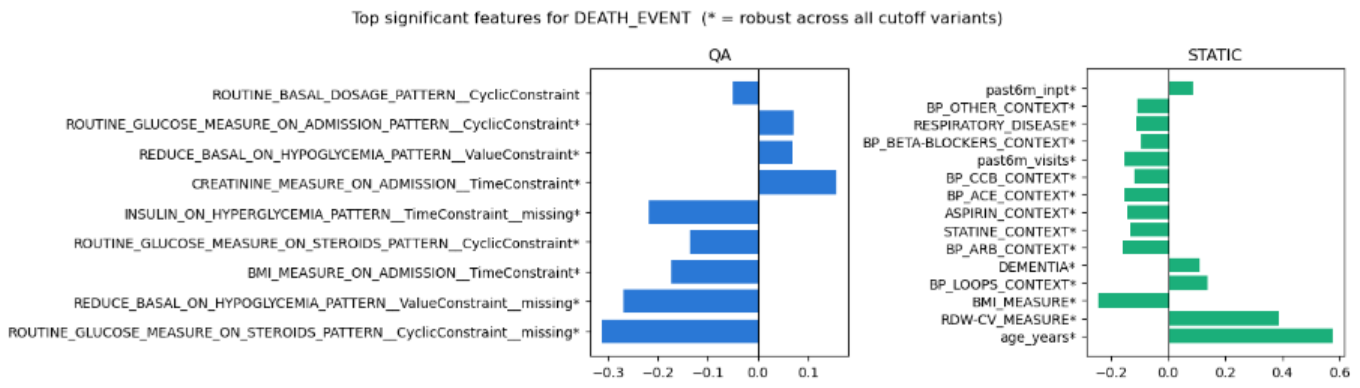
\includegraphics[width=\textwidth]{figures/death_feature_importance.png}
    \caption{
    Retained feature profile for 30-day mortality. The left panel shows
    retained guideline-adherence (QA) features and the right panel shows
    retained baseline clinical variables. Bar direction indicates the sign
    of the regression coefficient, while bar magnitude reflects the
    relative contribution after FDR correction and correlation pruning.
    Features marked with an asterisk persisted across all three
    observation-window definitions.
    }
    \label{fig:death-importance}
\end{figure}

\subsubsection{Recurring Guideline Recommendations Across Clinical Outcomes}

Synthesizing the adherence features across all outcome models
(Figure~\ref{fig:recurring-guidelines}), insulin following hyperglycemia and
admission glucose monitoring recurred most broadly, followed by BMI and
creatinine assessment on admission and monitoring during corticosteroid
treatment; basal-dose components appeared in fewer, more outcome-specific
models. Direction was not uniform---the same component could carry opposite
signs for different endpoints.

\begin{figure}[t]
    \centering
    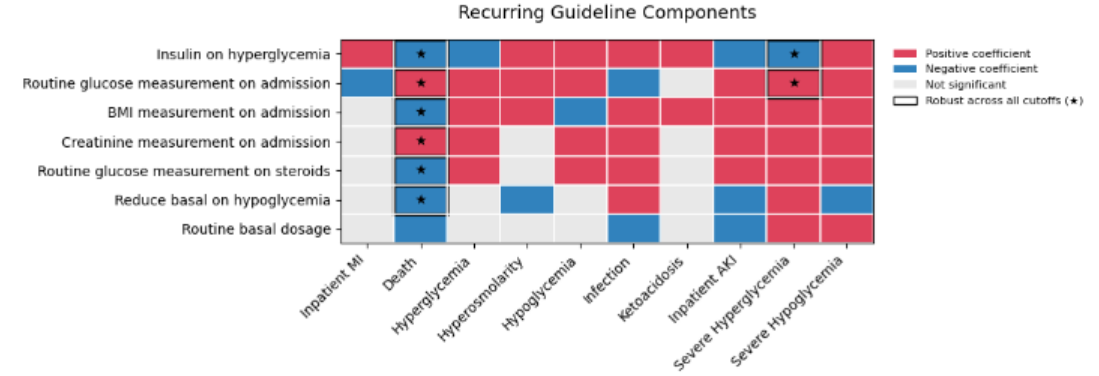
\includegraphics[width=\textwidth]{figures/recurring_guideline_components.png}
    \caption{
    Recurring guideline-adherence components identified by the bias-reduced
    regression models across clinical outcomes. Rows correspond to guideline
    recommendations and columns to clinical outcomes. Colored cells indicate
    statistically significant associations after FDR correction
    (red: positive regression coefficient; blue: negative regression
    coefficient). Stars denote associations that remained significant with
    a consistent direction across all three observation-window definitions
    (24, 48, and 72 hours). Blank cells indicate no statistically significant
    association.
    }
    \label{fig:recurring-guidelines}
\end{figure}

\subsection{Propensity-Weighted Evaluation of Guideline Adherence}

Because these models quantify conditional predictive associations rather
than treatment effects, both overall adherence and the recurrent components
were re-evaluated using inverse probability of treatment weighting (IPTW),
contrasting admissions above the median adherence score with those at or
below it. The overall-adherence analyses achieved satisfactory covariate
balance (maximum post-weighting standardized mean difference $<0.08$).

\subsubsection{Overall Guideline Adherence}

Relative to the low-adherence group, above-median adherence carried 44\%
lower odds of 30-day mortality (OR $=0.557$, 95\% CI $[0.514, 0.603]$),
82\% lower odds of hyperglycemia (OR $=0.175$, 95\% CI $[0.154, 0.199]$) and
52\% lower odds of severe hyperglycemia (OR $=0.485$, 95\% CI
$[0.450, 0.523]$), all FDR-adjusted $p<0.001$, against 20\% higher odds of
hypoglycemia (OR $=1.204$, 95\% CI $[1.090, 1.331]$, $p<0.001$;
Table~\ref{tab:iptw-overall}). Nothing survived correction for inpatient
myocardial infarction (MI), hyperosmolarity, infection, ketoacidosis or
inpatient acute kidney injury (AKI).

The asymmetry between those two directions is the substantive result: the
reduction in hyperglycemic burden is roughly ninefold larger on the log-odds
scale than the accompanying increase in hypoglycemia, and the increase in
\emph{severe} hypoglycemia did not reach significance (OR $=1.129$,
$p_{\mathrm{FDR}}=0.096$).

\subsubsection{Individual Guideline Recommendations}

We next examined the recurrent guideline recommendations identified above
using separate IPTW models (Table~\ref{tab:iptw-patterns}).
Only a subset of the recurrent predictors remained significant after
propensity weighting, indicating that several predictive associations were
largely explained by differences in baseline patient characteristics.

Of the significant associations, a further six were set aside because
propensity weighting failed to achieve acceptable covariate balance
(maximum post-weighting SMD between $0.90$ and $2.46$, against a
prespecified threshold of $0.10$). All six concerned BMI or creatinine
measurement on admission, for which adherence is near-universal
(mean $0.87$ and $0.98$ respectively, both with median $1.00$), so that
dichotomizing at the median produces groups too dissimilar to balance. The
corresponding coefficients were numerically degenerate and are not
interpretable; these component--outcome pairs are therefore reported as
non-estimable rather than as findings.

Eight associations were both significant and adequately balanced.
Above-median adherence to routine basal insulin dosing (OR $=0.748$),
routine glucose monitoring (OR $=0.870$) and insulin administration
following hyperglycemia (OR $=0.907$) each remained associated with lower
30-day mortality. For glycemic outcomes, insulin following hyperglycemia
(OR $=0.220$, 78.0\% lower odds) and routine basal insulin dosing
(OR $=0.402$, 59.8\% lower odds) were associated with substantially lower
odds of subsequent severe hyperglycemia, while insulin following
hyperglycemia also carried 28.3\% higher odds of hypoglycemia
(OR $=1.283$)---the same trade-off seen at the level of overall adherence.

These are the same components that showed the largest implementation gaps.
Insulin following hyperglycemia (mean adherence $0.15$) and routine basal
insulin dosing ($0.21$--$0.23$) are simultaneously the least-implemented
recommendations assessed and, after weighting, among those most strongly
associated with mortality and with severe hyperglycemia.

Adherence to glucose monitoring on admission was associated with a higher
recorded incidence of hyperglycemia (OR $=2.664$) and severe hyperglycemia
(OR $=2.121$). Since these outcomes are ascertained from glucose
measurements, more frequent early measurement mechanically increases the
chance of recording an event, so both associations likely reflect
ascertainment rather than harm. This component was retained, unlike routine
monitoring throughout the admission, which was excluded from the glycemic
models because it overlaps the detection window directly rather than being
bounded to the first days.

\begin{table}[t]
\centering
\caption{Inverse probability of treatment weighting (IPTW) analysis of
overall guideline adherence. Adherence was dichotomized at the median of
each outcome's eligible population; coefficients from the weighted logistic
regression models are therefore log-odds ratios comparing the above-median
with the at-or-below-median adherence group, and OR $=\exp(\beta)$ is the
corresponding odds ratio. Confidence intervals are unadjusted; $p$-values
were adjusted across outcomes using the Benjamini--Hochberg false discovery
rate (FDR) procedure. Covariate balance was assessed using the maximum
standardized mean difference (SMD) after weighting. MI, myocardial
infarction; AKI, acute kidney injury.}
\label{tab:iptw-overall}

\small
\setlength{\tabcolsep}{4pt}

\begin{tabular}{lrrrrr}
\toprule
Outcome & $\beta$ & OR & 95\% CI (OR) & Max SMD & $p_{\mathrm{FDR}}$ \\
\midrule
Hyperglycemia
    & $-1.742$ & 0.175 & [0.154, 0.199] & 0.019 & $<0.001$ \\

Severe hyperglycemia
    & $-0.724$ & 0.485 & [0.450, 0.523] & 0.012 & $<0.001$ \\

30-day mortality
    & $-0.586$ & 0.557 & [0.514, 0.603] & 0.020 & $<0.001$ \\

Hypoglycemia
    & $0.186$ & 1.204 & [1.090, 1.331] & 0.034 & $<0.001$ \\

Severe hypoglycemia
    & $0.121$ & 1.129 & [1.001, 1.274] & 0.030 & 0.096 \\

Hyperosmolarity
    & $0.106$ & 1.112 & [0.652, 1.896] & 0.020 & 0.800 \\

Ketoacidosis
    & $0.116$ & 1.123 & [0.561, 2.246] & 0.021 & 0.800 \\

Inpatient MI
    & $0.055$ & 1.057 & [0.732, 1.523] & 0.020 & 0.800 \\

Infection
    & $-0.025$ & 0.975 & [0.809, 1.175] & 0.020 & 0.800 \\

Inpatient AKI
    & $0.018$ & 1.018 & [0.888, 1.168] & 0.022 & 0.800 \\

\bottomrule
\end{tabular}
\end{table}

\begin{table}[t]
\centering
\caption{Inverse probability of treatment weighting (IPTW) analysis of
individual guideline recommendations. Rows are the component--outcome pairs
that were both statistically significant after FDR correction and adequately
balanced after weighting (maximum standardized mean difference
$<0.10$). Adherence to each recommendation was dichotomized at the median of
its eligible population, so coefficients compare above-median with
at-or-below-median adherence and OR $=\exp(\beta)$. Confidence intervals are
unadjusted; $p$-values were adjusted using the Benjamini--Hochberg false
discovery rate (FDR) procedure. A further six significant associations, all
concerning BMI or creatinine measurement on admission, failed the balance
criterion (maximum SMD $0.90$--$2.46$) and are not reported.
$^{\dagger}$Likely to reflect ascertainment rather than harm: the outcome is
detected from glucose measurements, so more frequent early measurement
increases the opportunity to record an event.}
\label{tab:iptw-patterns}

\small
\setlength{\tabcolsep}{4pt}

\begin{tabular}{llrrrr}
\toprule
Outcome & Recommendation & $\beta$ & OR & 95\% CI (OR) & $p_{\mathrm{FDR}}$ \\
\midrule

30-day mortality & Routine basal dosage
    & $-0.291$ & 0.748 & [0.691, 0.809] & $<0.001$ \\

30-day mortality & Routine glucose monitoring
    & $-0.139$ & 0.870 & [0.809, 0.937] & $<0.001$ \\

30-day mortality & Insulin after hyperglycemia
    & $-0.098$ & 0.907 & [0.842, 0.977] & 0.011 \\

\midrule

Severe hyperglycemia & Insulin after hyperglycemia
    & $-1.514$ & 0.220 & [0.202, 0.239] & $<0.001$ \\

Severe hyperglycemia & Routine basal dosage
    & $-0.912$ & 0.402 & [0.372, 0.434] & $<0.001$ \\

Severe hyperglycemia & Admission glucose monitoring$^{\dagger}$
    & $0.752$ & 2.121 & [1.974, 2.280] & $<0.001$ \\

\midrule

Hyperglycemia & Admission glucose monitoring$^{\dagger}$
    & $0.980$ & 2.664 & [2.389, 2.971] & $<0.001$ \\

\midrule

Hypoglycemia & Insulin after hyperglycemia
    & $0.249$ & 1.283 & [1.163, 1.416] & $<0.001$ \\

\bottomrule
\end{tabular}
\end{table}
